%%---------------------------------------------------------------------------%%
%% draco-3_2_0.tex
%% Thomas M. Evans
%% $Id$
%%---------------------------------------------------------------------------%%
\documentclass[note]{ResearchNote_pdf}
%\documentclass[11pt]{nmemo}
\usepackage[centertags]{amsmath}
\usepackage{amssymb,amsthm,graphicx}
\usepackage[mathcal]{euscript}
\usepackage{tmadd,tmath}
\usepackage{cite}
\usepackage{tabularx}
\usepackage{c++}
\usepackage{color}
\usepackage{float} % used for C++ example code.
\usepackage{shading}
\usepackage{fancybox}

%%---------------------------------------------------------------------------%%
%% DEFINE SPECIFIC ENVIRONMENTS HERE
%%---------------------------------------------------------------------------%%
%\newcommand{\elfit}{\ensuremath{\operatorname{Im}(-1/\epsilon(\vq,\omega)}}
%\msection{}-->section commands
%\tradem{}  -->add TM subscript to entry
%\ucatm{}   -->add trademark footnote about entry

\newcommand{\draco}{Draco}
\newcommand{\dracor}{\draco-3\_2\_0}
\newcolumntype{L}{>{\ttfamily}X}

\newcommand{\autoconf}{\textsf{Autoconf}}
\newcommand{\automake}{\textsf{Automake}} 
\newcommand{\CVS}{\textsf{CVS}}  
\newcommand{\make}{\textsf{Make}}

\newenvironment{codeExample}
{\footnotesize
  \VerbatimEnvironment
  \begin{SaveVerbatim}{\mycode}}%
  {\end{SaveVerbatim}%
  \noindent%
  \parashade[.950]{sharpcorners}{\gdef\outlineboxwidth{.5}%
    \UseVerbatim{\mycode}}\normalsize}

%%---------------------------------------------------------------------------%%
%% BEGIN DOCUMENT
%%---------------------------------------------------------------------------%%
\begin{document}

%%---------------------------------------------------------------------------%%
%% OPTIONS FOR NOTE
%%---------------------------------------------------------------------------%%

\toms{Distribution}
%\toms{Joe Sixpak/XTM, MS B226}
\refno{CCS--4:03-24(U)}
\subject{Release of \dracor}

%-------NO CHANGES
\divisionname{Computer and Computational Sciences Division}
\groupname{CCS-4:Transport Methods Group}
\fromms{Thomas M. Evans/CCS-4 D409}
\phone{(505)665--3677}
\originator{tme}
\typist{tme}
\date{7/25/2003}
%-------NO CHANGES

%-------OPTIONS
%\reference{NPB Star Reimbursable Project}
%\thru{P. D. Soran, XTM, MS B226}
%\enc{list}      
%\attachments{list}
%\cy{list}
%\encas
%\attachmentas
%\attachmentsas 
%-------OPTIONS

%%---------------------------------------------------------------------------%%
%% DISTRIBUTION LIST
%%---------------------------------------------------------------------------%%

\distribution {
  CCS--4, MS D409\\
  CCS--2, MS D413\\
}

%%---------------------------------------------------------------------------%%
%% BEGIN NOTE
%%---------------------------------------------------------------------------%%

\opening

\begin{abstract}
  We have released \dracor.  Although this is a minor \draco\ release,
  it contains some significant modifications to the Draco Build
  System.  These changes deal with vendors and compilation on ASCI
  White (IBM powerpc).  Also, some significant modifications to
  \draco\ packages are included in this release. We will summarize
  these changes in this release announcement. 
\end{abstract}

%%---------------------------------------------------------------------------%%

\section{\draco\ Contributors}

The following people are contributors to \draco:
\begin{center}
  \begin{tabular}{ll}
    Tom Evans & \texttt{tme@lanl.gov} \\
    Kelly Thompson & \texttt{kellyt@lanl.gov} \\
    Todd Urbatsch & \texttt{tmonster@lanl.gov} \\
    Kent Budge & \texttt{kgbudge@lanl.gov} \\
    Mike Buksas & \texttt{mwbuksas@lanl.gov} \\
    Jim Warsa & \texttt{warsa@lanl.gov} \\
    Rob Lowrie & \texttt{lowrie@lanl.gov} \\
    Todd Adams & \texttt{bta@lanl.gov} \\
    Paul Batcho & \texttt{batcho@lanl.gov} \\
  \end{tabular}
\end{center}

%%---------------------------------------------------------------------------%%

\section{\draco\ Component Packages}

\dracor\ contains the following component packages:
\begin{center}
  \begin{tabularx}{\linewidth}{
      >{\setlength{\hsize}{.5\hsize}}L %
      >{\setlength{\hsize}{1.5\hsize}}X}    
    \hline\hline 

    c4 & communication library \\
    cdi & Common Data Interface (CDI) component \\
    cdi\_analytic & CDI analytic data component \\
    cdi\_eospac & CDI EOSPAC wrapper \\
    cdi\_gandolf & CDI GANDOLF wrapper \\
    ds++ & data structures library \\
    imc & Implicit Monte Carlo physics component \\ 
    lapack\_wrap & wrapper to BLAS and LAPACK \\
    mc & Monte Carlo physics component \\
    meshReaders & mesh reader interface \\
    meshReaders\_Services & services for mesh readers (connectivity,
    etc) \\ 
    pcgWrap & wrapper for PCGLIB \\
    plot2D & 2-D plotter interface built on XMGRACE \\
    quadrature & quadrature component \\
    rng & random number generators and SPRNG wrappers \\
    RTT\_Format\_Reader & \texttt{meshReaders} implementation for RTT
    format meshes \\
    stdheaders & C-standard libraries wrapped in the \texttt{std::}
    namespace \\ 
    timestep & a timestep controller component \\
    traits & traits used by other \draco\ components \\
    units & a physics units component \\
    viz & interfaces to visualization tools (EnSight)\\
    xm & glommable expression templates \\  

    \hline\hline 
  \end{tabularx}
\end{center}
The following table summarizes changes to \draco\ components since
\draco-3\_1\_0. 
\begin{center}
  \begin{tabularx}{\linewidth}{
      >{\setlength{\hsize}{.5\hsize}}L %
      >{\setlength{\hsize}{1.5\hsize}}X}    
    \hline\hline 
    
    mc & added surfaces \\
    imc & surface tally tracking added to gray and multigroup
    particles\\
    cdi & added Rosseland integrators\\
    RTT\_Format\_Reader & general improvements\\
    c4 & DBC and testing added to \texttt{Timer} class\\

    \hline\hline 
  \end{tabularx}
\end{center}

There are no inter/intra-component cyclic dependencies in \draco.  The
levelized graph for \dracor\ components is shown in
Fig.~\ref{fig:level}.
\begin{figure}
  \label{fig:level}
  \centerline{
    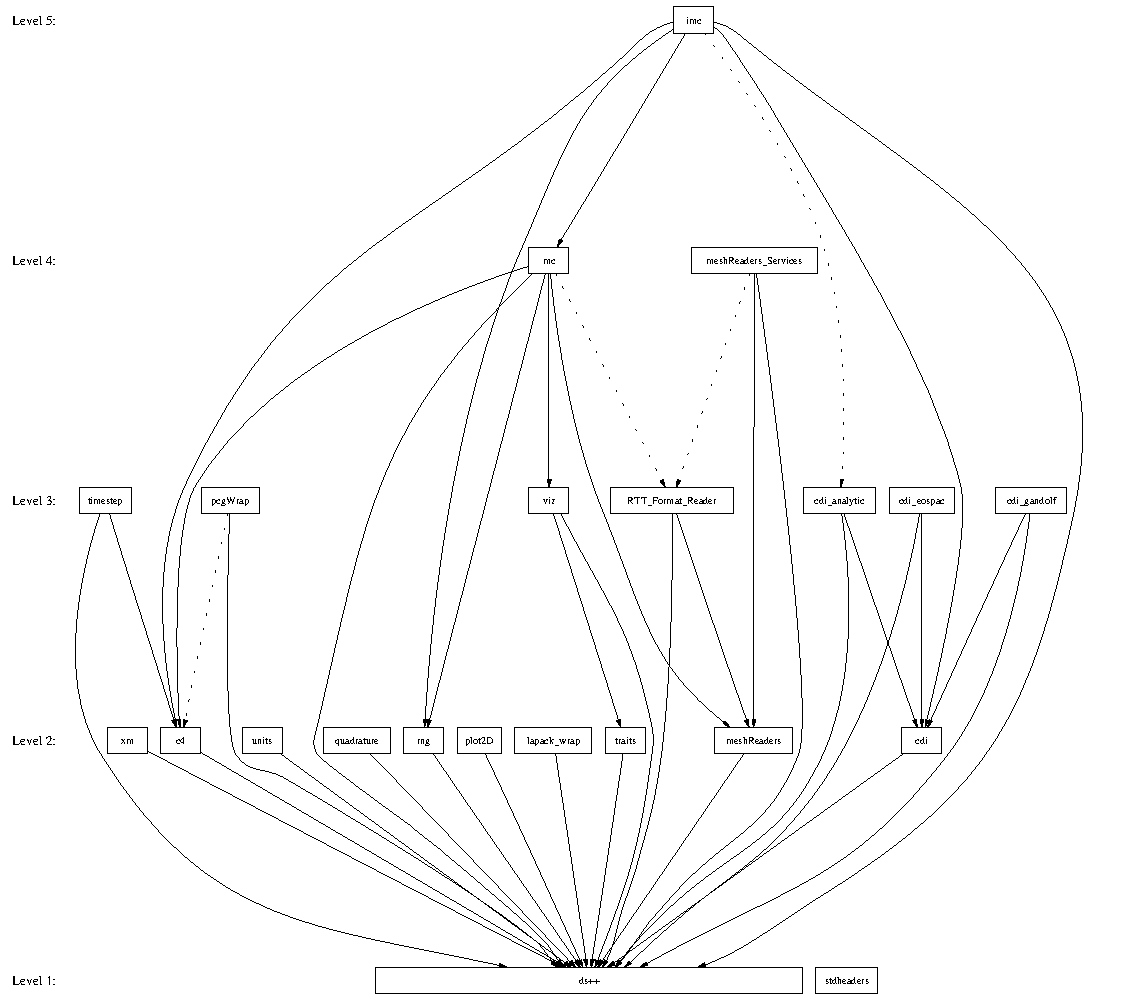
\includegraphics[height=5.5in]{level-3_0_0}}
  \caption{\dracor\ levelized component graph.  Dotted lines signify
    that the dependency if only required for testing.}
\end{figure}

Lines-of-Code (LOC) statistics for the component packages in \dracor\ 
are shown in Fig.~\ref{fig:stats}.  The aggregate LOC statistics for
\dracor\ are:
\begin{center}
  \begin{tabular}{|l|l|} \hline
    Total component package source code & 17534 \\
    Total unit test code & 20909 \\
    Total DBC statements & 2024 \\
    Total comments & 38139 \\
    \hline
  \end{tabular}
\end{center}
\begin{figure}
  \label{fig:stats}
  \centerline{
    \includegraphics[width=6in]{loc-3_2_0}}
  \caption{LOC statistics for \dracor\ component packages.}
\end{figure}

LOC metrics are stored in \draco\ in \texttt{draco/doc/code\_stats}.

%%---------------------------------------------------------------------------%%

\section{\draco\ Build System}

The \draco\ Build System (DBS) has undergone several changes.  First,
we have finally finished updates to the build system that allows
compilation on ASCI White.  Second, we have made significant internal
changes to the \texttt{ac\_vendors.m4} file.  Some of these changes
will affect DBS clients. 

\subsection{Building \draco\ on ASCI White}

Building \C++ code on ASCI White with a GNU-compliant build system
(\autoconf, \make) has proven difficult.  The difficulties are
twofold: the non-standard nature of IBM-AIX and the user-interface on
ASCI White.  We will not delve into great detail here; instead, we
will mention salient points about the ASCI White environment for the
purposes of archival record.

The vendor supplied IBM-AIX \C++ compiler is the Visual Age compiler, 
\texttt{xlC}.  However, ASCI White is configured to use compiler
scripts.  The serial compiler script is \texttt{newxlC} and the
MPI-based script is \texttt{newmpxlC}.  The DBS supports two
\texttt{--with-cxx} options:
\begin{verbatim}
     --with-cxx=asciwhite
     --with-cxx=ibm
\end{verbatim}
The \texttt{asciwhite} option is the default on IBM-AIX systems and
uses the script versions of the compilers. 

The following guidelines should be followed when compiling on ASCI
White:
\begin{itemize}
\item Use the DBS defaults whenever possible.
\item Do {\bf not} use \texttt{--with-mpi-inc} or
  \texttt{--with-mpi-lib} with the \texttt{asciwhite} compiler
  option.  The scripts automatically include MPI-related paths and
  libraries.  Trying to specify the libraries manually will almost
  certainly result in link/runtime errors.  To get a parallel build
  simply specify \texttt{--with-c4=mpi} on the configure line.
\item Because \texttt{CXX} is different for MPI-based and serial
  packages, do not use cache when configuring.  This is the default
  behavior (the cache option is specified by \texttt{-C} on the
  configure line).
\end{itemize}
Finally, we note that the IBM Visual Age compiler is somewhat flaky.
We do not recommend using White as a development platform.  Errors are
very hard to pin down and, in all cases so far, have been
compiler/linker bugs.  The IBM compiler support person at Livermore,
John Gyllenhaal \texttt{<gyllen@llnl.gov>}, (925) 424-5485, is very
helpful.

We have not tested all \draco\ components on ASCI White.  Only \draco\
components required for Wedgehog have been built and tested.
Additionally, some tests (e.g. \texttt{tstPingPong} in c4) will not
build because of compiler bugs.  This is an example of ASCI White
pathology, the same lines of code will compile in some translation
units but not in others.  We will hopefully get these issues worked
out over time.

\subsection{Build System Changes for Vendors}

We have significantly changed the internal workings of the DBS for
treating vendors.  Each vendor now has two macros:
\texttt{AC\_<vendor>\_SETUP} and \texttt{AC\_<vendor>\_FINALIZE}.
Details on these macros will be added to the inline build system
documentation.  For examples of the macros see \texttt{AC\_SPRNG\_SETUP}
and \texttt{AC\_SPRNG\_FINALIZE}.  

The impact of these changes for clients of the DBS is twofold:
\begin{enumerate}
\item The include paths are no longer stored inside of \draco\
  \texttt{config.h} files; thus, clients will need to add include
  paths at configure time.
\item The macro variables \texttt{VENDOR\_H} are no longer defined by
  the build system.  Instead include paths are appended to
  \texttt{CPPFLAGS}.  \draco\ components that use vendors have been
  modified to reflect this change.
\end{enumerate}
We will look at each of these issues in more detail.

Consider a client that uses the \draco\ \textsc{rng} package.
\textsc{rng} uses the SPRNG library.  A standard configure line for
\draco\ that contains \texttt{rng} might be the following:
\begin{verbatim}
     $ $draco_src/configure --prefix=/home/tme/build 
       --with-sprng-inc=/codes/radtran/vendors/sprng/include
       --with-sprng-lib=/codes/radtran/vendors/sprng/Linux/lib
\end{verbatim}
In previous versions of the DBS, the SPRNG include path was stored
inside of \texttt{rng/config.h}.  Thus, a client that used
\texttt{rng} did not have to specify a SPRNG include path, ie.
\begin{verbatim}
     $ $wedgehog_src/configure --prefix=/home/tme/build --with-draco
       --with-sprng-lib=/codes/radtran/vendors/sprng/Linux/lib
\end{verbatim}
Now, however, the include paths are no longer stored in the component
\texttt{config.h} files.  With \dracor\ we now have to add include
paths when configuring clients,
\begin{verbatim}
     $ $wedgehog_src/configure --prefix=/home/tme/build --with-draco
       --with-sprng-inc=/codes/radtran/vendors/sprng/include
       --with-sprng-lib=/codes/radtran/vendors/sprng/Linux/lib
\end{verbatim}
The result of this change is that we have to propagate information
about both library and include path locations for vendors to \draco\
clients. 

The second change affects code that uses vendors defined in the DBS.
In the past the DBS substituted the full include path plus header file
name into the \texttt{config.h} files for each component.  Consider
the \textsc{rng} component \texttt{config.h.in} file,
\begin{codeExample}
/* SPRNG library include path */
#undef SPRNG_H
\end{codeExample}
In the \textsc{rng}/SPRNG example from the preceding paragraph,
configure would expand \texttt{config.h.in} as follows:
\begin{codeExample}
/* SPRNG library include path */
#define SPRNG_H "/codes/radtran/vendors/sprng/include/sprng.h"
\end{codeExample}
This substition is no longer done in \dracor.  Instead, the include
path is added to \texttt{CPPFLAGS}.  The result of this change is that
components that relied on header file substitution will now have to
explicitly add the vendor headers to their source files.  In
\textsc{rng} this could be accomplished by modifying the file
\texttt{rng\_sprng.h} from 
\begin{codeExample}
#ifndef rtt_rng_rng_sprng_h
#define rtt_rng_rng_sprng_h

/* get the rng configuration file */
#include <rng/config.h>

/* Sprng Headers */
#include SPRNG_H

#endif                          /* rtt_rng_rng_sprng_h */
\end{codeExample}
to
\begin{codeExample}
#ifndef rtt_rng_rng_sprng_h
#define rtt_rng_rng_sprng_h

/* get the rng configuration file */
#include <rng/config.h>

/* Sprng Headers */
#include <sprng.h>

#endif                          /* rtt_rng_rng_sprng_h */
\end{codeExample}
We include the \texttt{sprng.h} header file explicitly instead of
through \texttt{CPP} macro substitution.  

%%---------------------------------------------------------------------------%%

\nocite{rn98046}
\nocite{xtm:9936}
\nocite{draco-3_0_0}
\bibliographystyle{rnote}
\bibliography{draco}
 
\closing
\end{document}

%%---------------------------------------------------------------------------%%
%% end of draco-3_2_0.tex
%%---------------------------------------------------------------------------%%
